\chapter{Cost-sensitive decision trees}\label{ch:7}

\begin{remark}{Outline}
In this chapter, we introduce the decision tree algorithm in Section \ref{sec:7:dt}. Then, in 
Section \ref{sec:7:csdt}, we described our previously proposed cost-sensitive decision tree. For 
this, we first shown the new cost-sensitive impurity measure, that introduces the diferent costs 
when evaluating the performance of a split. Then, we introduce a new cost-sensitive pruning 
criteria. Finally, in Section \ref{sec:7:experiments}, we compare the results of the proposed 
algorithm, against state-of-the-art methods, using the five real-world cost-sensitive databases.
\end{remark}

\section{Decision trees}
\label{sec:7:dt}

Decision trees are one of the most widely used machine learning algorithms \citep{Lior2008}. 
The technique is considered to be white box, in the sense that is easy to interpret, and has a 
very low computational cost, while maintaining a good performance as compared with more complex 
techniques \citep{Hastie2009}. There are two types of decision tree depending on the objective of 
the model. They work either for classification or regression. In this section we focus on
binary classification decision tree.

\subsection{Construction of classification trees}

Classification trees is one of the most common types of decision tree, in which the objective 
is to find the $Tree$ that best discriminates between classes. In general the decision tree 
represents a set of splitting rules organized in levels in a flowchart structure.

\subsubsection{Splitting criteria}

In the $Tree$, each rule is shown as a node, and it is represented as $(\mathbf{x}^j,l^j)$, meaning 
that the 
set $\mathcal{S}$ is split in two sets $\mathcal{S}^l$ and $\mathcal{S}^r$ according to 
$\mathbf{x}^j$ and $l^j$:
\begin{equation}
  \mathcal{S}^l = \{\mathbf{x}^a_i \vert \mathbf{x}^a_i \in \mathcal{S} \wedge x^j_i \le l^j \},
\end{equation}
and
\begin{equation}
  \mathcal{S}^r = \{\mathbf{x}^a_i \vert \mathbf{x}^a_i \in \mathcal{S} \wedge x^j_i > l^j \},
\end{equation}
where $\mathbf{x}^j$ is the $j^{th}$ feature represented in the vector 
$\mathbf{x}^j=[x_1^j,x_2^j,...,x_N^j]$, and $l^j$ is a value such that $min(\mathbf{x}^j) \le l^j < 
max(\mathbf{x}^j)$. Moreover, $\mathcal{S} = \mathcal{S}^l \cup \mathcal{S}^r$.

After the training set have been split, the percentage of positives in the different sets is 
calculated. First, the number of positives in each set is estimated by
\begin{equation}
 \mathcal{S}_1 = \{\mathbf{x}^a_i \vert \mathbf{x}_i^a \in \mathcal{S} \wedge y_i =1 \},
\end{equation}
then the percentage of positives is calculates as
\begin{equation}
 \pi_1=\vert \mathcal{S}_1 \vert / \vert \mathcal{S} \vert.
\end{equation}

Then, the impurity of each leaf is calculated using either a misclassification error, 
entropy or Gini measures:
\begin{itemize}
 \item  Misclassification
 \begin{equation}
 I_m(\pi_1)=1-max(\pi_1,1-\pi_1)
 \end{equation}
 
 \item Entropy
 \begin{equation}
 I_e(\pi_1)=-\pi_1\log \pi_1 -(1-\pi_1) \log (1-\pi_1)
 \end{equation}
 
 \item Gini
 \begin{equation}
 I_g(\pi_1)=2\pi_1(1-\pi_1)
 \end{equation}
\end{itemize}

In \figurename{ \ref{fig:7:impurity}}, the three measures are shown. All measures are similar, with 
the exception that the gini index and the cross-entropy are differentiable, which makes them
more suitable for numerical optimization.
\begin{figure}[t!]
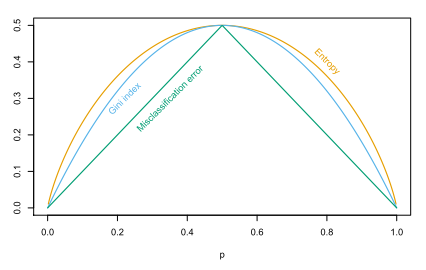
\includegraphics[scale=0.85]{ch7_fig1}
\caption{Impurity measures for a binary classification, as a function of the proportion of
positive examples in the set (Cross-entropy is scaled) \citep{Hastie2009}.}
\label{fig:7:impurity}
\end{figure} 

Finally the gain of the splitting criteria using the rule $(\mathbf{x}^j,l^j)$ is calculated as the 
impurity of $\mathcal{S}$ minus the weighted impurity of each leaf:
\begin{equation}\label{eq:7:gain}
  Gain(\mathbf{x}^j,l^j)=I(\pi_1)-\frac{\vert \mathcal{S}^l \vert}{\vert \mathcal{S} 
\vert}I(\pi^l_1)  -\frac{\vert \mathcal{S}^r \vert}{\vert \mathcal{S} \vert}I(\pi^r_1),
\end{equation} 
where $I(\pi_1)$ can be either of the impurity measures $I_e(\pi_1)$ or $I_g(\pi_1)$.

Subsequently, the gain of all possible splitting rules is calculated. The rule with maximal 
gain is selected
\begin{equation}
  (best_x, best_l) = \argmax_{(\mathbf{x}^j,l^j)}Gain(\mathbf{x}^j,l^j),
\end{equation}
and the set $\mathcal{S}$ is split into $\mathcal{S}^l$ and $\mathcal{S}^r$ according to that rule. 


\subsubsection{Tree growing}
In order to grow a tree typical algorithms use a top-down induction using a greedy search in each
iteration \citep{Rokach2010}. In each iteration, the algorithms evaluates all possible splitting 
rules and pick the one that maximizes the splitting criteria. After the selection of a splitting 
rule, each leaf is further selected and it is subdivides into smaller leafs, until one of the 
stopping criteria is meet. In Algorithm \ref{alg:7:tree_grow}, the pseudocode of the tree 
growing procedure is presented.

\begin{algorithm}\label{alg:7:tree_grow}
Pseudocode of the tree growing procedure.
\textnormal{
\begin{algorithmic}[1]
\Function{TreeGrow}{$\mathcal{S}$}
    \State $Tree = Empty$
    \If{\Call{Stopping}{$Tree, \mathcal{S}$}}
      \State \Return $Tree$
     \EndIf
    \State \# For all features
    \For{$j=1 \  to \ k$}
      \State \# For all possible thresholds
      \For{$m=1 \ to N_k$}
        \State $Gains(j,m) = $ \Call{Gain}{$\mathbf{x}^j,l^j_m, \mathcal{S}$}
      \EndFor
    \EndFor
    \State \# Select the threshold with the highest gain
    \State $(j^*, l^*) = argmax_{(j,m)}Gains$
    \State \# Split the set using the best rule
    \State $\mathcal{S}^l = \{\mathbf{x}^a_i \vert \mathbf{x}_i^a \in \mathcal{S} 
            \wedge \mathbf{x}_i^{j^*} \le l^* \}$
    \State $\mathcal{S}^r = \{\mathbf{x}^a_i \vert \mathbf{x}_i^a \in \mathcal{S} 
            \wedge \mathbf{x}_i^{j^*} > l^* \}$
    \State \# Recursively continue growing tree
    \State \Call{TreeGrow}{$\mathcal{S}^l$}
    \State \Call{TreeGrow}{$\mathcal{S}^r$}
    \State \# Return the tree
    \State \Return $Tree$
\EndFunction
\end{algorithmic}
}
\end{algorithm}

  
\subsubsection{Stopping criteria}
As the growing phase of the algorithm continue, at each iteration the stopping criteria are 
evaluated \citep{Rokach2010}. The most common stopping criteria are:
 \begin{itemize}
   \item All examples in the set belong to the same class. Meaning that either $\pi_1=1$ or 
    $\pi_1=0$.

  \item The maximum number of iterations have been reached.
  
  \item The number of examples in $\mathcal{S}$ are less than the minimum number of examples 
defined for a split.
  
  \item The number of examples in $\mathcal{S}^l$ or $\mathcal{S}^r$ are less than the minimum 
number of examples defined for a leaf.
  
  \item The best splitting rule has a Gain lower than a defined threshold.
\end{itemize}


\subsubsection{Pruning techniques}
After a decision tree has been fully grown, there is the big chance that  the algorithm generates a 
large tree that is probably over fitting the  training data. In order to solve this in 
\citep{Breiman1984a} originally suggest the use of pruning techniques after the tree growing phase.
The overall objective of pruning is to eliminate branches that are not contributing
to the generalization accuracy of the \mbox{tree \citep{Rokach2010}.}
 
In general pruning techniques start from a fully grown tree, and recursively check if by eliminating 
a $Branch$ there is an $Improvement$ in the error rate $\epsilon$ of the $Tree$.  There are two main 
methods to calculate the $Improvement$ of the error rate $\epsilon$ of the $Tree$, cost-complexity 
and  error based pruning:
  
\begin{itemize}
\item Cost-complexity pruning:
  
Initially proposed by Breiman  \citep{Breiman1984a}, this method evaluate iterative if the removal 
of a $Branch$ improve the error rate $\epsilon$ of a $Tree$, weighted by the difference of the 
number of leafs trees.
\begin{equation}\label{eq:7:pruning}
PC_{cc} = \frac{\epsilon(EB(Tree,branch),S)-\epsilon(Tree,\mathcal{S}) }
{\vert Tree\vert-\vert EB(Tree,branch)\vert}
\end{equation} 
where $\epsilon(Tree,\mathcal{S})$ calculate the error rate of the $Tree$ in set $\mathcal{S}$ and 
$EB(Tree,branch)$ is an auxiliary function that removes $branch$ from $Tree$ and return a new 
$Tree$. At each iteration, the current $Tree$ is compared against all possible $Branches$.
    
\item Error based pruning:
  
This method proposed by Quinlan  \citep{Quinlan1992} is more pessimistic and instead of  using the 
error rate $\epsilon$ calculate the upper bound of the confidence interval   of the error 
$\epsilon_{UB}$ calculated assuming a normal distribution with a defined significance level 
$Z_\alpha$.
\begin{equation}
PC_{eb} = \frac{\epsilon_{UB}(EB(Tree,branch),\mathcal{S})-\epsilon_{UB}(Tree,\mathcal{S}) }
    {\vert Tree\vert-\vert EB(Tree,branch)\vert}
\end{equation} 
where 
\begin{align}
    \epsilon_{UB}(Tree,&\mathcal{S})= \epsilon(Tree,\mathcal{S}) & \nonumber \\
    &+Z_\alpha \sqrt{  
\frac{\epsilon(Tree,\mathcal{S})(1-\epsilon(Tree,\mathcal{S}))}{\vert \mathcal{S} \vert}} &
\end{align}   
Moreover, as a difference from cost-complexity pruning, in the error based method, at each 
iteration not all the branches are compared, but only the ones on the same level. Meaning leafs 
are only compared against other leafs that are in the same level of iterations when the $Tree$ 
was constructed. This allows for much faster pruning procedure.
\end{itemize}

In Algorithm~\ref{alg:7:tree_pruning}, the general method of pruning is shown. The pruning 
procedure consists in evaluating the $Improvement$ of eliminating all possible branches in a $Tree$, 
and then eliminate the one with the higher $Improvement$ and repeat the process until a stopping 
criteria is meet.

\begin{algorithm}\label{alg:7:tree_pruning}
Pseudocode of the tree pruning procedure.
\textnormal{
\begin{algorithmic}[1]
\Function{TreePruning}{$\mathcal{S}, Tree$}
    \State \# For all branches
    \For{$branch \  in \ Tree.branches$}
      \State \# Evaluate the pruning criteria
      \State $Improvements(branch) = $ \Call{PC}{$\mathcal{S}, Tree, branch$}
    \EndFor
    \State \# Select the branch to prune
    \State $branch^* = argmax_{branch} Improvements$
    \State \# Prune selected branch
    \State $Tree = $ \Call{EB}{$TreeTree,branch^*$}
    \State \# Recursively continue pruning the tree
    \State \Call{TreePruning}{$\mathcal{S}, Tree$}
    \State \Return $Tree$
\EndFunction
\end{algorithmic}
}
\end{algorithm}

 
\subsubsection{Categorical features}
When using continuous features the splitting is done by testing all possible thresholds on the 
database and  selecting the one that maximizes the desired measure. Nevertheless, this is not 
straight forward when using a  categorical feature, since testing all possible ways of binning the 
feature becomes prohibitively time  consuming the feature has many categories. Instead, a common 
method for doing this is to calculate $\pi_1$ of each category, then sort it, and applied the 
method as a continuous feature \citep{Marslan2009}.



\subsection{Decision tree algorithms}
% \begin{remark}{Decision tree algorithms}
Two main branches of decision trees has being studied in the last years. The main difference is 
the  impurity measure used when splitting. First the CART algorithm that is based in the Gini 
index, and  later the ID3 and C4.5 which uses the entropy measure.

\begin{itemize}
 \item 
  CART or classification and regression trees was introduced by Brieman et al. in 1984 
\citep{Breiman1984a}. It is based on using the Gini index as the impurity measure and the tree is 
grow until all examples in  each leaf belong to the same class. Afterwards, the tree is pruned using 
the cost-complexity  method \citep{Rokach2010,Marslan2009}.
  
\item ID3
  algorithm uses entropy as the impurity measure. The growing of the tree stop when all 
examples belong  of each leaf belongs to the same class. In ID3 no pruning is applied 
\citep{Quinlan1992}.
  
\item C4.5
  the extension of ID3 both proposed by Quinlan \citep{Quinlan1992}.  Both are similar 
regarding the measure used, but C4.5 define the stopping criteria during the growth process
  to be when the number of examples in a set is less than a threshold. Moreover, after the tree is 
created  a error based pruning is applied \citep{Rokach2010}.
\end{itemize} 
% \end{remark}


\section{Example-Dependent Cost-sensitive Decision Trees}
\label{sec:7:csdt}

Standard decision tree algorithms focus on inducing trees that maximize accuracy. However this is 
	not optimal when the misclassification costs are unequal \citep{Elkan2001}. This has led to many 
	studies that develop algorithms that aim to introduce the cost-sensitivity into the algorithms 
	\citep{Lomax2013}. These studies have focused on introducing the class-dependent costs  
	\citep{Draper1994,Ting2002,Ling2004,Li2005,Kretowski2006,Vadera2010}, which is not optimal for 
	some applications. For example in credit card fraud detection, it is true that false positives 
	have a different cost than false negatives, nevertheless, false negatives may vary significantly, 
	which makes class-dependent cost-sensitive methods not suitable for this problem.
      
  In this section, we first propose a new method to introduce the costs into the decision tree 
	induction stage, by creating new-cost based impurity measures. Afterwards, we propose a new 
	pruning method based on minimizing the cost as pruning criteria.

	\subsection{Cost-sensitive impurity measures}

		Standard impurity measures such as misclassification, entropy or Gini, take into account the 
		distribution of classes of each leaf to evaluate the predictive power of a splitting rule,
		leading to an impurity measure that is based on minimizing the misclassification rate. However, 
		as has been previously shown \citep{CorreaBahnsen2013}, minimizing misclassification does not 
		lead to the same results than minimizing cost. Instead, we are interested in measuring how good 
		is a splitting rule in terms of cost not only accuracy. For doing that, we propose a new 
		example-dependent cost based impurity measure that takes into account the cost matrix of each 
		example.

		We define a new cost-based impurity measure taking into account the costs when all the examples
		in a leaf are classified both as negative using $f_0$ and positive using $f_1$
		\begin{equation}\label{eq:cost_impurity}
			I_c(\mathcal{S}) = \min \bigg\{ Cost(f_0(\mathcal{S})), Cost(f_1(\mathcal{S})) \bigg\}.
		\end{equation}
		The objective of this measure is to evaluate the lowest expected cost of a splitting rule.
		Following the same logic, the classification of each set is calculated as the prediction that 
		leads to the lowest cost
	  \begin{equation}\label{eq_pred}
	    f(\mathcal{S}) = 
	    \begin{cases}
	      \phantom{-}0 \phantom{-} \mbox{if} \phantom{-} Cost(f_0(\mathcal{S})) \le 
        Cost(f_1(\mathcal{S}))\\
	      \phantom{-}1 \phantom{-}\mbox{otherwise}
	    \end{cases}
	  \end{equation}

		Finally, using the cost-based impurity, the splitting criteria cost based gain of using the 
		splitting rule $(\mathbf{x}^j,l^j)$ is calculated with (\ref{eq:7:gain}). 

	\subsection{Cost-sensitive pruning}
 
		Most of the literature in class-dependent cost-sensitive decision tree focuses on using the 
		misclassification costs during the construction of the algorithms \citep{Lomax2013}. Only few 
		algorithms such as AUCSplit \citep{Ferri2002} have \mbox{included} the costs both during and 
		after the construction of the tree. However, this approach only used the class-dependent costs, 
		and not the example-dependent costs.
 
		We propose a new example-dependent cost-based impurity measure, by replacing the error rate 
		$\epsilon$ in (\ref{eq:7:pruning}) with the cost of using the $Tree$ on $\mathcal{S}$ i.e. by 
    replacing with 	$Cost(f(\mathcal{S}))$.
		\begin{equation}\label{eq:cost_pruning}
			PC_{c} = \frac{ Cost(f(\mathcal{S})) - Cost(f^*(\mathcal{S})) }
		  {\vert Tree\vert-\vert EB(Tree,node)\vert} ,
		\end{equation}
		where $f^*$ is the classifier of the tree without the selected node $EB(Tree,node)$.
 
		Using the new pruning criteria, nodes of the tree that do not contribute to the minimization of 
		the cost will be pruned, regardless of the impact of those nodes on the accuracy of the
		algorithm. This follows the same logic as in the proposed cost-based impurity measure, since 
		minimizing the misclassification is different than minimizing the cost, and in several 
		real-world applications the objectives align with the cost not with the misclassification error.
		
\section{Experiments}
\label{sec:7:experiments}

\todo{complexity}
